\makeatletter
\def\input@path{{../../}}
\makeatother
\documentclass[../../main.tex]{subfiles}

\graphicspath{
	{../../img/}
	{../img/}
	{img/}
}

\begin{document}
\section{Двойной интеграл ( 2 И ) }

Рассмотрим Ф2П $ f \left( x, y \right) $  , где 
$ \left( x, y \right) \in D \subset \R^n $ и $ D $ - измеримое множество 
в $ \R^2 $ (плоская квадрируемая фигура). В этом случае имеем \emph{2И}:

\begin{equation}
	\label{lec_13, num_12}
	I = \iint\limits_{D} f \left( x, y \right)  dxdy
\end{equation}

\begin{thm}[О вычислении 2И по прямоугольнику для 
непрерывных Ф2П]
    Пусть $ f \left( x, y \right)  $ - непрерывна на прямоугольнике
    $ \text{П} = \left[\ a, b\ \right] \times \left[\ c, d\ \right] =  \left\lbrace \ 
    \left( x, y \right) \in \R^2\ |\ a \leq x \leq b, \ c \leq y \leq d\ \right\rbrace $.
    Тогда для \eqref{lec_13, num_12} $ \implies $
    \begin{equation}
    \label{lec_13, num_13}
    I = \int\limits_a^b \left( \int\limits_c^d f \left( x, y \right) dy  \right) dx =
     \int\limits_c^d \left( \int\limits_a^b f \left( x, y \right) dx  \right) dy
    \end{equation}
\end{thm}

\begin{proof}
	Рассмотрим произвольное разбиение $ \widetilde{P} = 
	\left\lbrace x_i \right\rbrace  $, $i = \overline{1,m} $ 
	отрезка $ \left[ a, b\right]  $. T.e $a = x_0 < x_1 < \dots 
	< x_{i-1} < x_i < \dots < x_m = b $. Пусть $ \overline{P} $
	 - разбиение точками $ \left\lbrace y_j \right\rbrace  $, 
	 где $j = \overline{1, l} $ отрезка $ \left[ c, d\right]  $. 
	 T.e $c = y_0 < y_1 < \dots < y_{j-1} < y_j < \dots < y_l = d $.
	 
	 С помощью вертикальных прямых $ x = x_i $, $ i = \overline{1, m} $
	 и горизонтальных прямых $ y = y_j $, $ j = \overline{1, l} $
	 прямоугольник $ \text{П} $ разобъется на части: $ \text{П}_{ij} = 
	 \left[ x_{i - 1}, x_i \right] \times \left[ y_{i - 1}, y_i \right] $, образующим
	 соответствующее разбиение $ P = \left\lbrace \text{П}_{ij} \right\rbrace $,
	 $ i = \overline{1, m} $, $ j = \overline{1, l} $ исходного $ \text{П} $. Т.е. 
	 $ \text{П} = \bigcup\limits_{i = 1}^m \bigcup\limits_{j = 1}^l \text{П}_{ij}$, 
	 которые могут иметь общими лишь граничные точки
	 
	 \begin{center}
	 	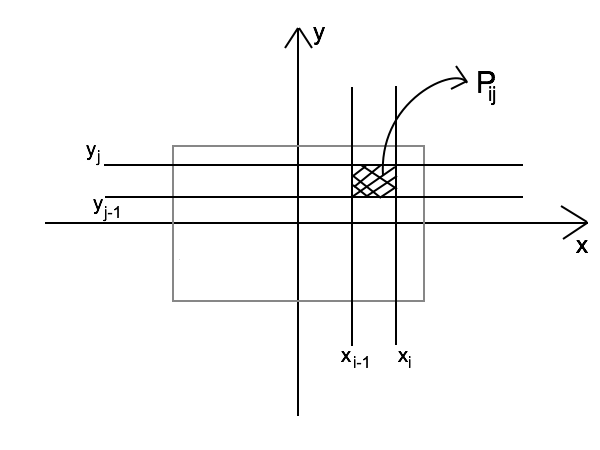
\includegraphics[width=0.6\textwidth]{lec13_rectangle.png}
	 \end{center}
 
 	Т.к $ f \in C( \text{П} )$ (т.е непрерывна), то $ f \in C( \text{П}_{ij} )$,
 	$ \forall i = \overline{1, m} , \forall j = \overline{1, l}$. Для каждого 
 	$ fix\ i = \overline{1, m} $ рассмотрим функцию $ F_i \left( y \right) = 
 	\int\limits_{ x_{i - 1} } ^ {x_i} f \left( x, y \right) dx $, $ i = \overline{1, m} $
 	
 	Эта функция корректно определена, т.к $ \forall fix\ y \implies f \left( x, y\right) $
 	непрерывна по $ x \implies $ интегрируема по $ x $. По теореме о среднем
 	для однократных интегралов $ \implies \exists t_{ij} \in \left[ x_{i - 1}, x_i \right] $, 
 	т.ч $ F_j \left( y_j \right) = \int\limits_{x_{i - 1} } ^ {x_i} f \left( x, y_j \right) dx = 
 	f \left(  t_{ij}, y_j \right) \Delta x_i$, $ \Delta x_i = x_i - x_{i - 1}$, где 
 	$ i = \overline{1, m} $
 	
 	В соответствии с этим получаем множество $ Q = \left\lbrace M_{ij} \right\rbrace $,
 	где $ M_{ij} = \left( t_{ij}, y_j \right) \in \text{П}_{ij} $, $ i = \overline{1, m} $, 
 	$ j = \overline{1, l} $
 	
 	Т.к все используемые множества измеримы (квадрируемы в $ \R^2 $), 
 	то для полной \emph{специальной} интегральой суммы
 	\begin{equation}
 	\label{lec_13, num_14}
 	\sigma = \sigma \left( t, \left( P, Q \right) \right) = \sum\limits_{i = 1}^m 
 	\sum\limits_{j = 1}^l f \left( M_{ij} \right) \Delta \text{П}_{ij}
 	\end{equation}
 	где $\Delta \text{П}_{ij} = \Delta x_i \Delta y_j$ - площадь $\text{П}_{ij}$ 
 	( $ \Delta x_i = x_i - x_{i-1}, \Delta y_j = y_j - y_{j - 1} $ )
 	
 	Имеем:
 	\[ \sigma = \sum\limits_{i = 1}^m \sum\limits_{j = 1}^l f \left( M_{ij} \right) 
 	\Delta x_i \Delta y_j = \]
 	
 	\[ = \sum\limits_{j = 1}^l \sum\limits_{i = 1}^m F_i \left( y_j \right) \Delta y_j = 
 	\sum\limits_{j = 1}^l \left( 
 	\int\limits_{x_0 = a}^{ x_1 } + \int\limits_{x_1}^{ x_2 } + \dots + 
 	\int\limits_{ x_{m-1} }^{x_m = b} \right) \Delta y_j = \]
 	
 	\[ = \sum\limits_{j = 1}^l \left( \int\limits_a^b f \left( x, y_j\right) dx \right)
 	 \Delta y_j =  \]
 	
 	\begin{equation}
 	\label{lec_13, num_15}
 	= \sum\limits_{j = 1}^l F \left( y_j \right) \Delta y_j 
 	\end{equation}
 	
 	где
 	\begin{equation}
 	\label{lec_13, num_16}
 	\begin{cases}
 	F \left( y \right) = \int\limits_a^b f \left( x, y \right) dx \\
 	y \in \left[ c, d \right] 
 	\end{cases}
 	\end{equation}
 	
 	Из \eqref{lec_13, num_15} $ \implies $ что рассматриваемая $\sigma$
 	является одной из интегральных сумм для Ф1П  \eqref{lec_13, num_16}.
 	Отсюда при 
 	\[ \widetilde{d} = diam \widetilde{P} = 
 	max \left\lbrace \Delta y_j \right\rbrace \underset{1 \leq j \leq l}{\longrightarrow} 0 \]
 	В силу непрерывности, а значит интегрируемости получаем: 
 	\[ \exists \lim\limits_{ \widetilde{d} \to 0 } \sigma = 
 	\lim\limits_{ \widetilde{d} \to 0 } \sum\limits_{j = 1}^l F \left( y_j \right) \Delta y_j =
 	\int\limits_c^d F \left( y \right)dy  \]
 	
 	В силу непрерывности и интегрируемости с использованием
 	специальных интегральный сумм за счет выбора точек, предел $ \sigma $
 	будет такой же, как и предел общих интегральных сумм 
 	в силу критерия Гейне
 	
 	Таким образом получим, что
 	\[ I = \lim\limits_{ \widetilde{d} \to 0 } \sigma = \int\limits_c^d F \left( y \right) dy =  \]
 	\[ = \int\limits_c^d \left( \int\limits_a^b f \left( x, y\right) dx \right) dy \]
 	что соответсвует правой части \eqref {lec_13, num_13} 
 	
 	Аналогично доказывается равенство и в левой части \eqref {lec_13, num_13} 
\end{proof}




\begin{defn}[Коши]
    \[\forall \eps > 0 \quad \exists \delta > 0 \quad \forall x \in D(f) \quad
      0 < \abs{x-x_0} < \delta \implies \abs{f(x) - a} \le \eps\]
\end{defn}

\begin{thm}[Про \LaTeX]
    \LaTeX\ крут :)
\end{thm}

\begin{proof}
    По определению.
\end{proof}

\begin{crl}[\texttt{alex65536}]
    Электронный конспект стоит вести в \LaTeX'е.
\end{crl}

\begin{crl}
    \LaTeX-документы текстовые,
    поэтому можно использовать \texttt{git} для конроля версий.
\end{crl}

\begin{rem}
    Числовые множества в \LaTeX: $\R\C\Q\N\Z$.
\end{rem}

\begin{exmp}
    Пример примера :)
\end{exmp}


\begin{lem}[О единственном следствии из теоремы]
 Следствие может быть без номера (если оно одно)
\end{lem}

\begin{proof}
 Используйте \texttt{crl*}!
\end{proof}

\begin{crl*}
    Получится как-то так
\end{crl*}

\begin{exc}
    За\LaTeX'ать весь матан.
\end{exc}

\bigskip

Заметим, что строчки лучше делать короткими.
Так будет проще смотреть изменения.

\begin{exmp}[Маяковский]

    Такой текст

\begin{verbatim}
    Послушайте!
    Ведь, если звезды зажигают~--
    значит~-- это кому-нибудь нужно?
    Значит~-- кто-то хочет, чтобы они были?
    Значит~-- кто-то называет эти плевочки
                                  жемчужиной?
\end{verbatim}

    отформатируется как

    \medskip

    Послушайте!
    Ведь, если звезды зажигают~--
    значит~-- это кому-нибудь нужно?
    Значит~-- кто-то хочет, чтобы они были?
    Значит~-- кто-то называет эти плевочки
                                  жемчужиной?

\end{exmp}

\begin{thm}[Критерий]
 В критерии надо доказывать как необходимость, так и
 достаточность.
\end{thm}

\begin{proof}
 \quad

 \nec Необходимость критерия надо доказать!

 \suff Достаточность критерия тоже надо доказать!

\end{proof}

\end{document}
